\section{Inverter Sizing}
\label{Sect:2}

This section discusses the process of inverter selection and verification based on the motor's operational requirements and field weakening behavior. Two inverter options are considered: INV1 and INV2.

\subsection{Inverter Specifications}

The rated values for both inverters are reported below:

\begin{table}[!h]
    \centering
    \begin{tabular}{lcc}
        \toprule
        \textbf{Parameter} & \textbf{INV1} & \textbf{INV2} \\
        \midrule
        DC-Link Voltage $V_{dc}$ [V] & 480 & 400 \\
        Maximum Current $I_{\text{max}}$ [A] & 300 & 200 \\
        Base Speed $n_{\text{base}}$ [rpm] & \multicolumn{2}{c}{3406} \\
        Maximum Speed $n_{\text{max}}$ [rpm] & \multicolumn{2}{c}{15000} \\
        \bottomrule
    \end{tabular}
    \caption{Comparison between candidate inverters.}
    \label{tab:inverters}
\end{table}

\subsection{Driving Cycle Evaluation}

To verify the compatibility of each inverter, the required torque-speed points are evaluated over a representative driving cycle. As shown in Fig.~\ref{fig:inv_sizing}, INV2 is not sufficient to cover all required operating points. In contrast, INV1 satisfies the constraints across the full speed-torque range.

\begin{figure}[!h]
    \centering
    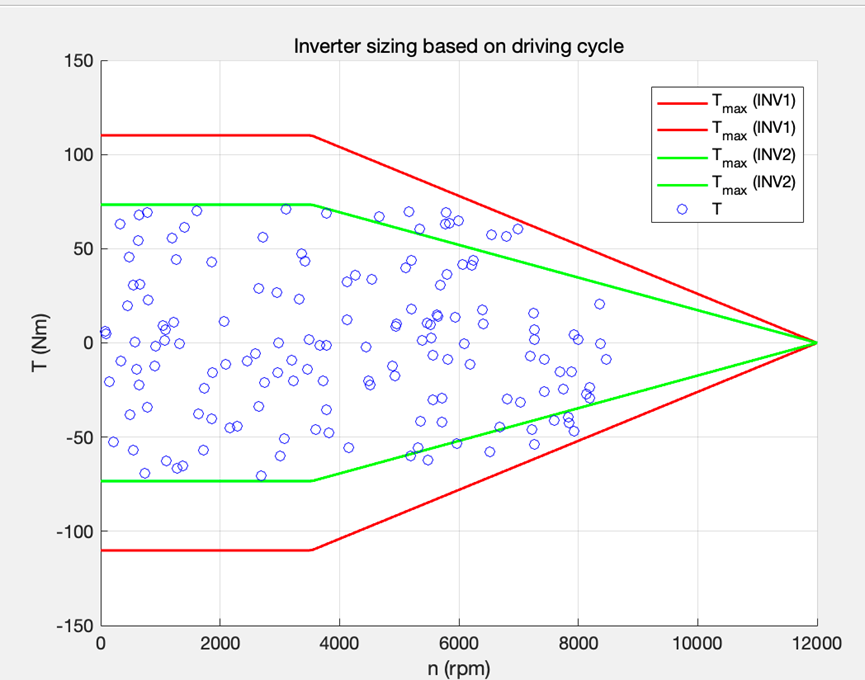
\includegraphics[width=0.8\linewidth]{Figures/Inverter sizing based on a driving cycle.png}
    \caption{Inverter sizing based on a driving cycle. INV2 is not able to cover all operation points, while INV1 is sufficient.}
    \label{fig:inv_sizing}
\end{figure}

\subsection{Field Weakening Analysis}

At speeds above base speed, field weakening (FW) is activated. This requires careful coordination between voltage and current limits.

Figure~\ref{fig:fw_max_current} shows the maximum current during FW (top) and the corresponding flux amplitude and torque (bottom). The inverter must support these current peaks without thermal or voltage breakdown.

\begin{figure}[!h]
    \centering
    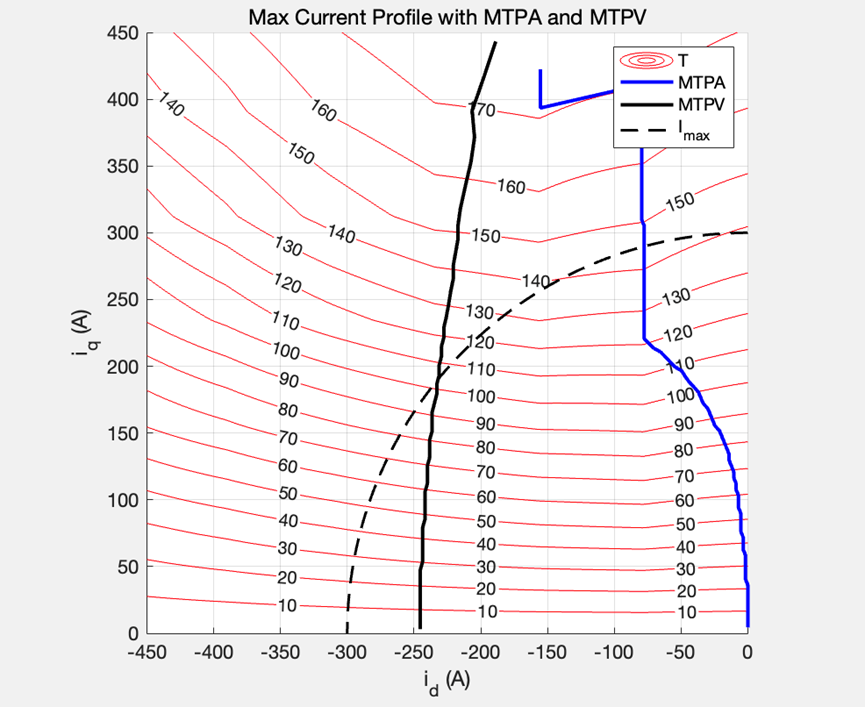
\includegraphics[width=0.8\linewidth]{Figures/Max current profile during FW.png}
    \caption{Maximum current profile during field weakening (top) and corresponding flux and torque (bottom).}
    \label{fig:fw_max_current}
\end{figure}

From the analysis, we conclude:

\begin{itemize}
    \item INV2 is insufficient for high-speed operation due to voltage and current limitations.
    \item INV1, with higher voltage and current capability, successfully covers all operational points including FW.
\end{itemize}

Therefore, **INV1 is selected** for further control and simulation steps.

